\chapter{Background}
 
\section{Database Management Systems}

Modern database management systems (DBMS) are complex software systems that provide a high-level interface for users to interact with the underlying data. DBMSs such as \textit{MySQL} \cite{mysqlwebpage} offer a large set of features, including data storage, retrieval and manipulation.

Relational DBMSs, usually exposing \textit{SQL} as a query language, form an overwhelming majority of the database systems in use today, with the 4 most popular DBMSs being relational \cite{akhtar2023popularity}. The relational model was introduced by Edgar Codd in $1970$ \cite{codd1970relational}, and offers application developers a high-level manipulation capacity of the stored data. Information is modeled as collections of relations between properties, commonly represented as tables and rows.

Modern \textit{SQL} offers a \textit{Data Definition Language} (DDL) to create and modify the structure of the underlying data, and a \textit{Data Manipulation Language} (DML) to interact with the data. The DDL is composed of statements such as \textit{CREATE} and \textit{DROP}, while DML is composed of statements such as \textit{SELECT}, \textit{INSERT}, \textit{UPDATE}, and \textit{DELETE}.

\section{Transactions}

A transaction is a sequence of instructions executed as a single isolated unit of work \cite{gray1981transaction}. In other words, either all of the instructions in the transaction are correctly executed and saved to the database, or none of them are. Transactions offer the ACID properties \cite{microsofttransaction}, a set of properties that guarantee that database transactions are processed reliably. The ACID properties are as follows:

\begin{itemize}
    \item \textbf{Atomicity}: A transaction is an atomic unit of work, meaning that the database will either execute all of the instructions in the transaction, or none of them.
    \item \textbf{Consistency}: A transaction will bring the database from one consistent state to another consistent state. In other words, the database will always be in a consistent state, regardless of the state of the running transactions.
    \item \textbf{Isolation}: Multiple transactions can be executed concurrently, and, depending on the isolation level, the transactions will not interfere with each other.
    \item \textbf{Durability}: Once a transaction is committed successfully, the DBMS guarantees that the changes made by the transaction will be saved to the database.
\end{itemize}


\section{Isolation Levels}

The isolation between transactions is defined by the isolation level. Stricter isolation levels~\cite{si,psi,serializability} offer more consistency guarantees, at the cost of performance~\cite{hat,noc-noc}; 
weaker isolation levels~\cite{ramp,lora,ua,tcc,DBLP:conf/fase/LiuOSWGM18,pc} cater for diverse real-world applications, such as social media. 
While many isolation levels have been formalized, the ANSI isolation levels supported by most database systems \cite{melton1992iso_ANSI} are as follows:

\begin{itemize}
    \item \textbf{Read Uncommitted}: The lowest isolation level. Transactions can read uncommitted data from other transactions.
    \item \textbf{Read Committed}: Transactions are visible only after being committed.
    \item \textbf{Repeatable Read}: Transactions are visible only after being committed, and multiple reads of the same data will return the same result. Note that new data can be become visible to the transaction.
    \item \textbf{Serializable}: The strongest (and slowest) isolation level, in which transactions can be assumed to be executed serially.
\end{itemize}

% Add the image `assets/adya_isolation_levels.png`.
\begin{figure}[H]
    \centering
    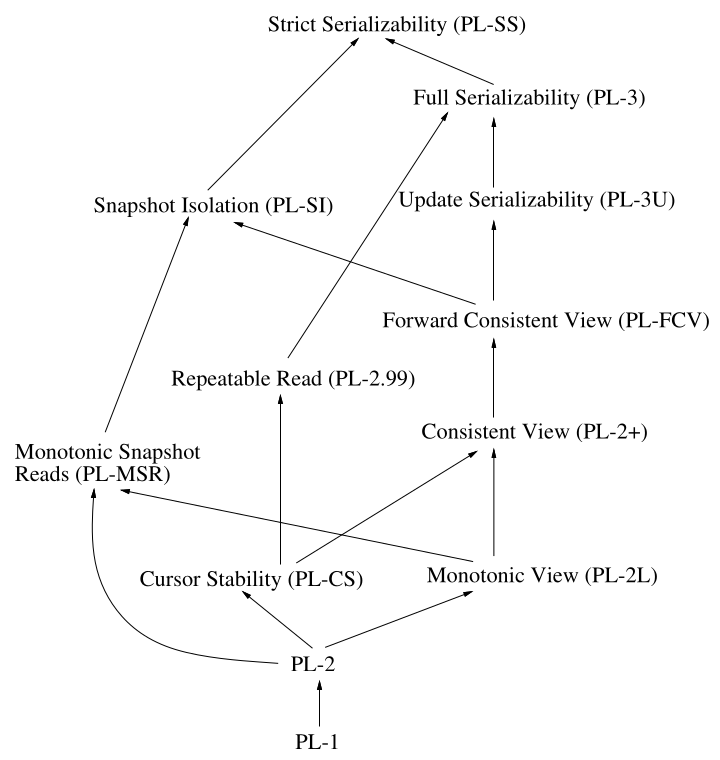
\includegraphics[width=0.7\textwidth]{assets/adya_isolation_levels.png}
    \caption{The Adya isolation levels \cite{adya1999weak}.}
    \label{fig:adya_isolation_levels}
\end{figure}

In modern DBMSs, the isolation levels are implemented by leveraging concurrency control techniques such as locking and multi-version concurrency control (MVCC). The choice of isolation level is a trade-off between consistency guarantees and concurrency performance, and is usually made by the application developer.

For instance, a banking application which needs to avoid double-spending will use the \textit{Serializable} isolation level, while a school grading system might want to use the \textit{Read Committed} isolation level.

\section{Transaction and Isolation Bugs}

DBMSs are complex software systems, with their complexity constantly increasing as diminishing returns push for more and more complex optimizations. Like all software, DBMSs are prone to bugs, which can lead to data corruption, loss of data, or crashes.

Transaction and isolation bugs are part of a specific class of bugs residing in the transaction and isolation handling mechanisms of a DBMS. Such bugs are tricky to detect, as they often require multiple concurrent transactions, might occur sporadically due to the nondeterministic nature of the concurrency, and might not be easily reproducible.

While similar, transactional and isolation bugs are slightly different:
\begin{itemize}
    \item \textbf{Transactional bugs}: Logic bugs that occur when one or multiple transactions are being run. Possible manifestations include unexpected failures, missing data, or incorrect behavior.
    \item \textbf{Isolation bugs}: Bugs that occur when the specified isolation level is not respected. Possible manifestations include forbidden behavior, such as dirty reads, non-repeatable reads, or phantom reads.
\end{itemize}

\section{Related Work}

The topic of database testing is not new, but has gained significant interest over the last few years, with multiple new techniques and tools developed to ensure the reliability and correctness of database management systems. At the core of this research field lies the need to detect, replicate and understand logical and transactional bugs (which affect the core functionality of the DBMS system, respectively which violate constrainsts imposed by the isolation level) \cite{biswas2019complexity}.

Recent work has focused on fuzzing techniques, based on the repeated checking of randomized testcases \cite{aflwebpage}, combined with novel methods of detecting errors in random transactions \cite{jiang2023detecting, cui2022differentially_ASE2022, dou2023detecting_ICSE2023, clark2024validating, kingsbury2020elle}. A recent paper by Cui, Z.\ et al. \cite{cui2024understanding_ICSE2024} makes a comprehensive survey of reported transactional bugs, a large portion discovered with the help of the before-mentioned fuzzing techniques.

Cui et al. proposed \textit{DT2}, a testing framework based on differential testing, a technique that compares the output of the same statements run on two different DBMSs \cite{cui2022differentially_ASE2022}. By generating random database states and executign concurrent transactions, \textit{DT2} was able to identify $10$ new bugs across \textit{MySQL}, \textit{MariaDB} and \textit{TiDB}. The choice of the DBMS systems picked for testing is not accidental, as they are some of the most popular DBMSs in use today, and \textit{MariaDB} and \textit{TiDB} are advertized as drop-in replacements for \textit{MySQL}.

From a different approach, Clark, J.\ et al. \cite{clark2024validating} proposed \textit{Emme}, a white-box testing framework for detecting isolation bugs by checking violations of the Adya dependency graph \cite{adya1999weak}. The bug-finding technique relies on existential constraints imposed on bug-valid traces of DBMS transactions, expressed as constraints on a directed graph. The tool relies on \textit{version certificate recovery}, a technique that injects versioning on database records, and \textit{version certificate validation}, a technique which extracts the Adya dependency graph from the versioned records. While the authors of the paper did not find any new bugs, they were able to validate the correctness of their approach by detecting manually injected bugs.

Similarely, Jiang, Z.\ et al. \cite{jiang2023detecting} proposed a novel technique for finding isolation bugs using SQL instrumentation. The technique relies on a similar approach to \textit{Emme}, but the idea of instrumenting SQL queries with additional checks allows the running the instrumented queries in a black-box fashion. The authors are unable to generate a sound Adya dependency graph, but are able to generate single transactions histories equivalent to concurrent ones, allowing for a differential-testing based approach. The authors were able to find $56$ new bugs in \textit{MySQL}, \textit{MariaDB} and \textit{TiDB}.

Other tools~\cite{kingsbury2020elle,tan2020cobra,viper,polysi,plume,isovista,cat} employ a large variety of techniques for finding bugs.
For instance,
the \textit{Elle} fuzzer restricts the writes to an append-only list, \cite{kingsbury2020elle}, while \textit{Cobra} relies on key-value stores and on the read-modify-write series of operations \cite{tan2020cobra}. However, such tools miss on the complexity of the SQL language (e.g. nested or ranged queries \cite{jiang2023dynsql}), and are usually unable to handle arbitrary SQL queries, notably those with sub-queries or sub-queries~\cite{levy1994query}.

Our work is inspired by the comprehensive surveying work of Cui, Z.\ et al. \cite{cui2024understanding_ICSE2024} on transactional bugs. The survey cataloged a wide range bugs across multiple DBMSs and reported from various fuzzing tools or simple database users, and captures recurring patterns. However, as the authors acknowledge, their analysis of bugs is "\textit{based on their issue descriptions, embedded test cases, developer discussions, and available fixing patches}", and, to the best of our knowledge, the authors of the survey did not actually replicate the collected bugs, due to constraints on the DBMS versions (often a Git commit) and time consumption.

In this work, we aim to build on the results of Cui, Z.\ et al. \cite{cui2024understanding_ICSE2024} by replicating a large subset of the transactional bugs reported in their survey, with a focus on isolation bugs. We aim to replicate the bugs in a controlled, container-based environment, and to understand the root cause of the bugs by analyzing the transaction histories.

In the second part of our project, as a follow-up to our findings, we also build on the work of Clark, J. et al. \cite{clark2024validating} which find bugs by checking violations of the Adya dependency graph \cite{adya1999weak} in a white-box fashion, and on the work of Jiang, Z. et al. \cite{jiang2023detecting} which introduces the novel idea of SQL instrumentation. Using these two techniques, we introduce a new technique for finding isolation bugs using Adya dependency graphs in a black-box fashion, leveraging the SQL instrumentation technique.
